% This file was created with tikzplotlib v0.9.16.
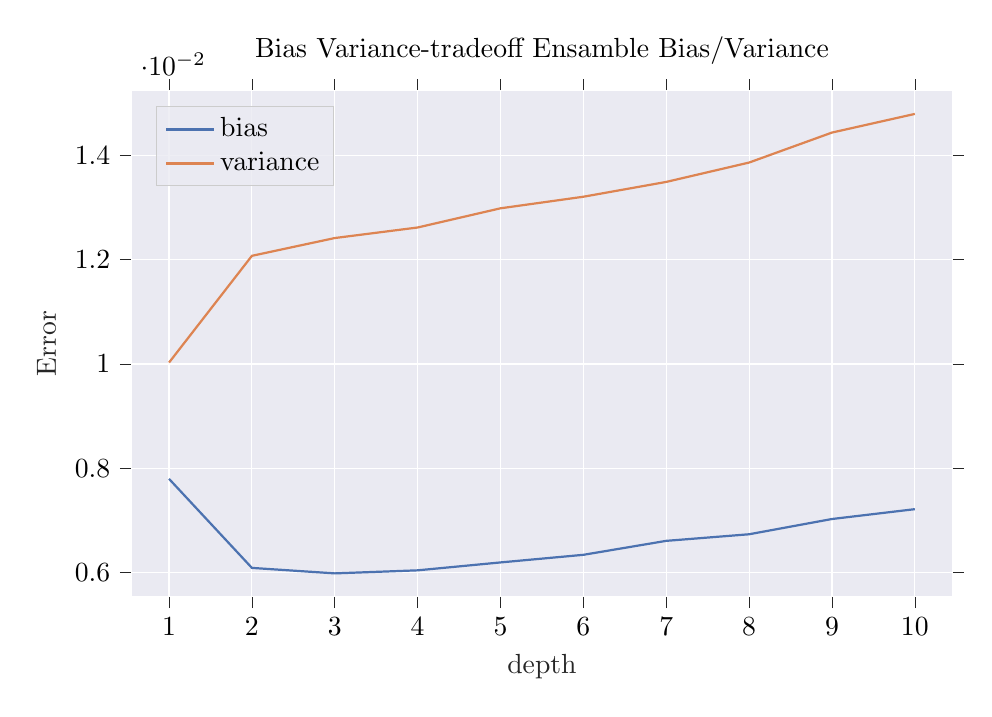
\begin{tikzpicture}

\definecolor{color0}{rgb}{0.917647058823529,0.917647058823529,0.949019607843137}
\definecolor{color1}{rgb}{0.298039215686275,0.447058823529412,0.690196078431373}
\definecolor{color2}{rgb}{0.866666666666667,0.517647058823529,0.32156862745098}

\begin{axis}[
width=12cm,height=8cm,axis background/.style={fill=color0},
axis line style={white},
legend cell align={left},
legend style={
  fill opacity=0.8,
  draw opacity=1,
  text opacity=1,
  at={(0.03,0.97)},
  anchor=north west,
  draw=white!80!black,
  fill=color0
},
tick align=outside,
title={Bias Variance-tradeoff Ensamble Bias/Variance},
x grid style={white},
xlabel=\textcolor{white!15!black}{depth},
xmajorgrids,
xmajorticks=true,
xmin=0.55, xmax=10.45,
xtick style={color=white!15!black},
y grid style={white},
ylabel=\textcolor{white!15!black}{Error},
ymajorgrids,
ymajorticks=true,
ymin=0.00554465145606449, ymax=0.0152374590610859,
ytick style={color=white!15!black}
]
\addplot [thick, color1]
table {%
1 0.0077977180480957
2 0.00609040260314941
3 0.00598526000976562
4 0.00604367256164551
5 0.0061953067779541
6 0.00634121894836426
7 0.00660896301269531
8 0.00673544406890869
9 0.00702798366546631
10 0.0072166919708252
};
\addlegendentry{bias}
\addplot [thick, color2]
table {%
1 0.010028600692749
2 0.0120754241943359
3 0.0124164819717407
4 0.0126186609268188
5 0.0129867792129517
6 0.0132086277008057
7 0.0134927034378052
8 0.0138640403747559
9 0.0144391059875488
10 0.0147968530654907
};
\addlegendentry{variance}
\end{axis}

\end{tikzpicture}
